% mn2esample.tex
%
% v2.1 released 22nd May 2002 (G. Hutton)
%
% The mnsample.tex file has been amended to highlight
% the proper use of LaTeX2e code with the class file
% and using natbib cross-referencing. These changes
% do not reflect the original paper by A. V. Raveendran.
%
% Previous versions of this sample document were
% compatible with the LaTeX 2.09 style file mn.sty
% v1.2 released 5th September 1994 (M. Reed)
% v1.1 released 18th July 1994
% v1.0 released 28th January 1994

\documentclass[useAMS,usenatbib]{mn2e}
\usepackage{graphicx}
\usepackage{journals}
\usepackage{amsmath}
\def\5{\footnotesize V\normalsize}
\def\4{\footnotesize IV\normalsize}
\def\3{\footnotesize III\normalsize}
\def\2{\footnotesize II\normalsize}
\def\1{\footnotesize I\normalsize}
\def\lam{$\lambda$}
\def\kms{$\mbox{km s}^{-1}$}
\def\p{$\phantom{:}$}
\def\a{$\phantom{^\ast}$}
\def\v{$\phantom{^{l}}$}
\def\pp{$\phantom{-}$}
\def\o{$\phantom{0}$}
\def\vr{$v_{\rm r}$}


% If your system does not have the AMS fonts version 2.0 installed, then
% remove the useAMS option.
%
% useAMS allows you to obtain upright Greek characters.
% e.g. \umu, \upi etc.  See the section on "Upright Greek characters" in
% this guide for further information.
%
% If you are using AMS 2.0 fonts, bold math letters/symbols are available
% at a larger range of sizes for NFSS release 1 and 2 (using \boldmath or
% preferably \bmath).
%
% The usenatbib command allows the use of Patrick Daly's natbib.sty for
% cross-referencing.
%
% If you wish to typeset the paper in Times font (if you do not have the
% PostScript Type 1 Computer Modern fonts you will need to do this to get
% smoother fonts in a PDF file) then uncomment the next line
% \usepackage{Times}

%%%%% AUTHORS - PLACE YOUR OWN MACROS HERE %%%%%


%%%%%%%%%%%%%%%%%%%%%%%%%%%%%%%%%%%%%%%%%%%%%%%%

\title[Dynamics and Metallicities in NGC\,2100]{Dynamics and Metallicities of Red Supergiant Stars in the Young Massive Cluster NGC\,2100}
\author[L. R. Patrick et al.]{L. R. Patrick$^{1}$\thanks{E-mail: lrp@roe.ac.uk}, C. J. Evans$^{1, 2}$, B. Davies$^{3}$, et al.\\
$^{1}$Institute for Astronomy, University of Edinburgh, Royal Observatory Edinburgh, Blackford Hill, Edinburgh EH9 3HJ, UK\\
$^{2}$UK Astronomy Technology Centre, Royal Observatory Edinburgh, Blackford Hill, Edinburgh EH9 3HJ, UK\\
$^{3}$Astrophysics Research Institute, Liverpool John Moores University, Liverpool Science Park ic2, 146 Brownlow Hill, Liverpool L3 5RF, UK
}

% \author[A. V. Raveendran and A. N. Other]{A. V. Raveendran$^{1}$\thanks{E-mail:
% email@address (AVR); otheremail@otheraddress (ANO)} and A. N.
% Other$^{2}$\footnotemark[1]\thanks{This file has been amended to
% highlight the proper use of \LaTeXe\ code with the class file.
% These changes are for illustrative purposes and do not reflect the
% original paper by A. V. Raveendran.}\\
% $^{1}$Indian Institute of Astrophysics, Bangalore 560034, India\\
% $^{2}$Building, Institute, Street Address, City, Code, Country}
\begin{document}

\date{Accepted  Received 1; in original form}

\pagerange{\pageref{firstpage}--\pageref{lastpage}} \pubyear{2015}

\maketitle

\label{firstpage}

\begin{abstract}
Studies of the dynamical state of young massive clusters can distinguish between models of early-time evolution.
We have obtained KMOS near-IR spectroscopy for 14 red supergiant stars in the young massive star cluster NGC\,2100 in the Large Magellanic Cloud (LMC).
Radial velocities are estimated for the targets and the dynamical properties are estimated for the first time within this cluster.
The line-of-sight velocity dispersion is shown to be flat outside of 10\,pc from the cluster centre and is estimated to be
$\sigma_{1D}~=~3.01\pm0.11\,$\kms.
The dynamical mass of the cluster is derived as
$log(M_{dyn}/M_{\odot})~>~4.8$ assuming virial equilibrium.
Comparing this to the mass estimated using photometry we find the dynamical mass to be a factor of five smaller.

Stellar parameters including metallicity are estimated using the $J$-band analysis technique which has been rigorously tested in the Local Universe.
The results of this analysis are shown to compare well with previous metallicity estimates within this cluster and to within the LMC in general.
The age of the NGC\,2100 is estimated to be $20\pm5\,$Myr using isochrone fitting to the RSG population, in good agreement with previous estimates.

\end{abstract}

\begin{keywords}
Red Supegiants: stars. Clusters: NGC\,2100. Galaxy: LMC.
\end{keywords}

\section{Introduction} % (fold)
\label{sec:introduction}

% Red supergiant stars (RSGs) have long been explotied to probe extragalactic environments.
% Owing to their intrinsic brightness and cool temperatures, these stars have a peak wavelength in the near-IR which makes RSGs ideal candidates to study extragalactic environments (refs).
Globular clusters (GCs) were until recently thought to consist of a simple stellar population where all of the stars within the cluster were formed from in one homogeneous star forming burst.
Recent results have thrown this traditional view into contention and many GCs have been shown to display an extended main-sequence turn off (ref!), double main sequences (ref!) as well as distinct chemical~\citep{2012A&A...539A..19G} and dynamical(ref!) populations.
The most accepted method to explain these observations is to evoke a GC with multiple stellar populations.

Young massive clusters are important probes of cluster evolution.
These custers have gained considerable attention within the past 20 years as tracers of star formation~\citep[e.g.][]{1995AJ....109..960W,1997AJ....114.2381M,1999AJ....118..752Z}.
Young massive clusters are thought to be younger counterparts to Globular Clusters.
Recently, GCs have been proposed to contain multiple stellar populations based on their kinematics, metallicities and main sequence turn-offs.
Studying young massive clusters can help to constrain some of the proposed models for creating multiple stellar populations within GCs.


\citet{2015A&A...575A..62N}, show that there exists no significant age spread in several young massive clusters within the LMC.
In recent years it has become clear that young massive clusters appear to remain in virial equilibrium from an early stage~\citep{2014prpl.conf..291L}.
This is in direct conflict with the formation scenario where star clusters are destroyed owing to gas expulsion~\citep[i.e. infant mortality,][]{2003ARA&A..41...57L}.

Over the last few years, medium resolution ($R~>~3000$) near-IR spectroscopy has been shown to be a powerful tool to estimate stellar parameters for red supergiant stars~\citep[RSGs;][]{2010MNRAS.407.1203D}.
This technique has been tested rigorousness by~\cite{2014ApJ...788...58G} and \cite{2015ApJ...806...21D} and demonstrated with data from the $K$-band multi-object spectrograph first in~\cite{2015ApJ...803...14P} who investigated the metallicity distribution within NGC\,6822 ($d~=~0.5\,Mpc$) then by
\cite{2015ApJ...805..182G} who compare the metallicity gradient derived within NGC\,300, a grand design spiral galaxy outside the Local Group ($d~=~1.9\,Mpc$), finding striking agreement with blue supergiant stars (BSGs).

Using multi-object spectrographs like KMOS to observe RSGs provides an efficient way to construct a sample of metallicity measurements in extragalactic stellar systems where one can study the distribution and build-up of metals within these systems.

% This analysis takes into account non-LTE affects for the strongest lines within a narrow region of the $J$-band~\citep{2012ApJ...751..156B,2013ApJ...764..115B,2015ApJ...804..113B} and estimates global metallicity ([Z]), effective tmperature (T$_{eff}$), surface gravity ($log,\,g$) and microturblence ($\xi$).

NGC\,2100 is a young massive cluster in the Large Magellanic Cloud (LMC), located near the large star forming region 30 Doradus.
With an age of $\sim$20\,Myr~\citep{1991ApJS...76..185E,2015A&A...575A..62N}, and a mass of $4.6~\times~10^4M_{\odot}$~\citep[assuming~\cite{1966AJ.....71...64K} profiles]{2005ApJS..161..304M}, NGC\,2100 falls within the mass and age range where the infrared cluster light is dominated by RSGs~\citep{2013MNRAS.430L..35G}.
This has been confirmed observationally where a large number of RSGs have been identified within this cluster.

NGC\,2100 is not a cluster in isolation.
It is located in one of the most actively star-forming regions within the Local Group of galaxies.
At $\sim$20\,Myr old, the most massive members of this star cluster have already gone supernova.
This has had a profound affect on the surrounding gas and dust, and has potentially shaped the surrounding LMC\,2 supershell~\citep[see][]{1999ApJ...518..298P}.



In this study we estimate stellar parameters from KMOS spectroscopy for 14 RSGs in the vicinity of the young massive cluster NGC\,2100.
Section~\ref{sec:observations} we describe the observations and data reduction, and in section~\ref{sec:results} we detail our results, focusing on radial velocities of the target stars where we derive the line-of-sight velocity dispersion, the dynamical mass of NGC\,2100 and the stellar parameters.
Our results are discussed in Section~\ref{sec:discussion} and conclusions are presented in Section~\ref{sec:conclusions}.



% Something great about the LMC and how NGC\,2100 fits into the mix.
% NGC\,2100 is a young massive star cluster located on the near edge of the LMC, near the 30 Dor region.
% There have been many studies which have identified a large number of RSGs within the cluster.
% This is the first quantitative estimate of their metallicities.

% Some NGC\,2100 stats:\\
% Age: 20\,Myr~\citep{2015A&A...575A..62N} \\
% Mass: $4.36\times10^{4}$~\citep{2005ApJS..161..304M}\\
% R$_{core}$ (pc): 3.03/0.99~\citep{2005ApJS..161..304M}\\
% Z: $log0.007/Z_{\odot} = -0.34$~\citep{2015A&A...575A..62N}\\
% V$_{esc}$ (\kms): 7.9~\citep{2005ApJS..161..304M}\\

% [Z] is first estimated in~\cite{1994A&A...282..717J} using




% Questions we would like to answer in this paper:\\
% Are the known RSGs in this region genuine cluster members and if so what does their velocity dispersion look like?\\

% How does the metallicity of these objects relate the to that in the nearby 30 Dor region and other RSGs within this galaxy?


% section introduction (end)

\section{Observations and Data Reduction} % (fold)
\label{sec:observations}
\subsection{Target Selection} % (fold)
\label{sub:target_selection}

\begin{itemize}
  \item Ben, could you write a few lines here?
\end{itemize}

\begin{figure}
 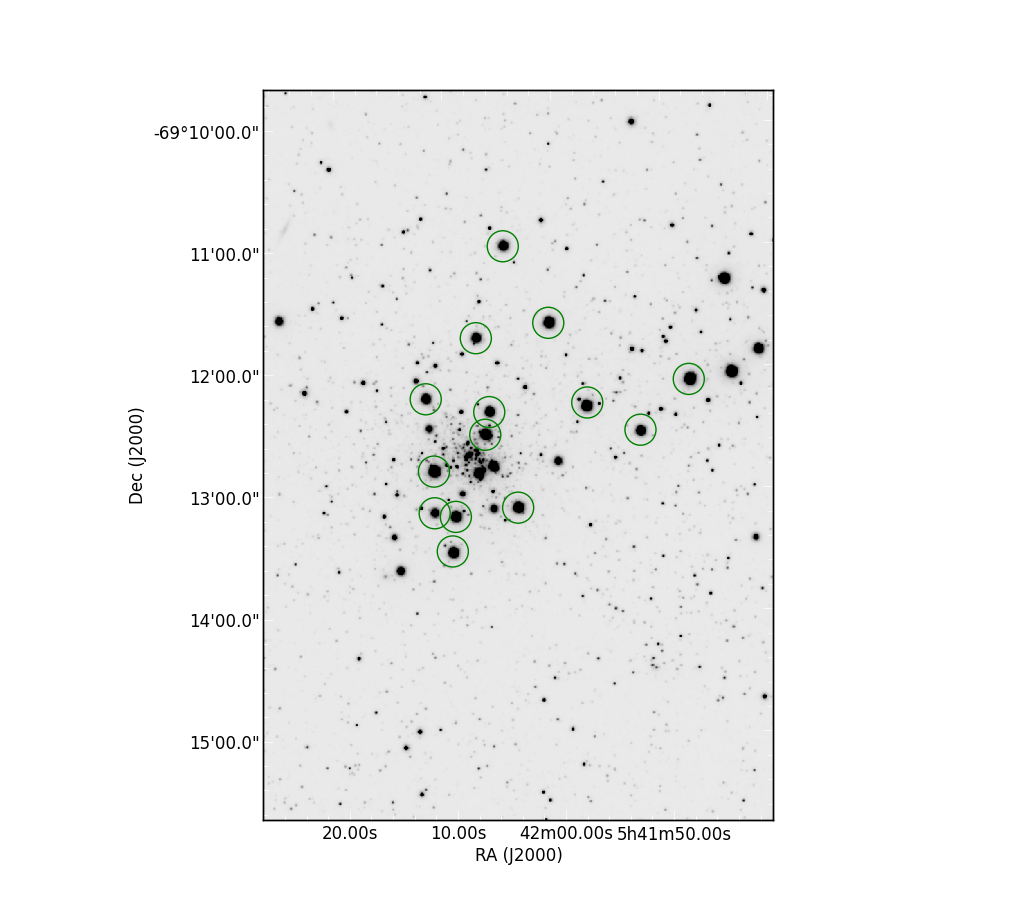
\includegraphics[width=9.0cm]{NGC2100-targets}
 \caption{Positions of the NGC\,2100 KMOS targets overlaid on a VISTA $J$-band image.
          Green circles indicate KMOS targets.
          The cluster centre has been marked by a small blue cross.
          \textbf{include 5pc marker!}
\label{fig:targets}
          }
\end{figure}

% subsection target_selection (end)
\subsection{KMOS Observations} % (fold)
\label{sub:kmos_observations}

% subsection kmos_observations (end)
These observations form part of the KMOS Guaranteed Time Observing (PI: Evans) and were conducted in March 2015.
The observations consist of $8\times10$\,s exposures taken with the YJ grating with sky offset exposures (S) interleaved between the object (O) exposures in an O,~S,~O observing pattern.
In addition, a standard set of KMOS calibrate frames were also obtained as well as telluric standard frames using HD\,51506 as the telluric standard star.
Seeing conditions were stable at 1.0\,arcseconds for the course of the observations.

The KMOS/esorex standard routines~\citep[SPARK;][]{2013A&A...558A..56D} were used to calibrate and reconstruct the data cubes.
Telluric correction was performed using the 24-arm telluric correction routine
~\citep[described in detail by][]{2015ApJ...803...14P}.
Briefly, corrections to the standard telluric recipe are put in place to correct for slight differences in wavelength calibration between the telluric and science spectra.
This is implemented using an iterative cross-correlation approach.
Additionally, differences in the strength of the telluric features are corrected by apply a simple scaling using the equation,

\begin{equation}
  T_{2} = (T_{1} + c) / (1 + c)
\end{equation}

\noindent where $T_{2}$ is the scaled telluric-standard spectrum, $T_{1}$ is the uncorrected telluric-standard spectrum and $c$ is the scaling parameter which is varied from $c~=~-0.5$ to $c~=~0.5$ in increments of 0.02.
The best $c$ value is chosen based on the overall standard deviation of the spectrum, i.e. the $c$ value producing the smallest $\sigma$ is selected.
Once these corrections are accounted for, the science spectra are divided by the appropriate telluric spectrum for that particular IFU.


\begin{table*}
\caption{
        Summary of VLT-KMOS targets in NGC\,2100.\label{tb:obs-params}
        }
\scriptsize
\begin{center}
\begin{tabular}{lrcccccccccl}
 \hline
 \hline
ID & S/N & $\alpha$ (J2000) & $\delta$ (J2000) & $B$ & $V$ & $I$ & $J$ & $H$ & $K_{\rm s}$ & RV (\kms) & Notes \\
 \hline
0207-0134568 & 318 & 05:41:47.873 & -69:12:05.959 & 16.488 & 13.749 &  9.769 &  9.525 &  8.603 & 8.200 & 238.9$\pm$1.1\\
0207-0134683 & 198 & 05:41:52.430 & -69:12:30.410 & 16.430 & 14.267 & 11.970 & 10.413 &  9.526 & 9.155 & 238.7$\pm$2.2\\
0207-0134811 & 202 & 05:41:57.286 & -69:12:16.480 & 14.074 & 13.019 & 11.170 &  9.811 &  9.036 & 8.738 & 239.8$\pm$1.3 & C2\\
0207-0134979 & 252 & 05:42:03.877 & -69:13:07.410 & 15.624 & 13.579 & 11.410 &  9.839 &  8.996 & 8.740 & 240.4$\pm$1.5\\
0207-0135059 & 196 & 05:42:06.348 & -69:12:20.150 & 00.000 & 00.000 & 11.810 & 10.371 &  9.480 & 9.159 & 245.0$\pm$2.9 & B17\\
0207-0135069 & 256 & 05:42:06.764 & -69:12:31.245 & 15.643 & 13.675 & 11.390 &  9.977 &  9.150 & 8.807 & 239.5$\pm$2.3\\
0207-0135150 & 240 & 05:42:09.647 & -69:13:11.263 & 15.367 & 13.383 & 11.370 &  9.976 &  9.136 & 8.841 & 240.8$\pm$3.2\\
0207-0135162 & 250 & 05:42:10.001 & -69:13:28.210 & 16.060 & 13.827 & 11.580 & 10.021 &  9.150 & 8.823 & 240.2$\pm$1.4 & C32\\
0207-0135205 & 304 & 05:42:11.574 & -69:12:48.770 & 16.327 & 14.033 & 11.450 &  9.557 &  8.617 & 8.264 & 238.0$\pm$1.9\\
0207-0135206 & 151 & 05:42:11.592 & -69:13:09.257 & 16.165 & 14.272 & 12.340 & 10.943 & 10.090 & 9.788 & 241.4$\pm$2.5\\
0207-0135220 & 195 & 05:42:12.182 & -69:12:13.144 & 15.483 & 13.606 & 11.750 & 10.440 &  9.622 & 9.335 & 246.0$\pm$3.3\\
0208-0135292 & 262 & 05:42:00.722 & -69:11:36.925 & 15.579 & 13.674 &  9.421 &  9.900 &  9.017 & 8.683 & 242.2$\pm$3.1\\
0208-0135383 & 211 & 05:42:04.762 & -69:10:58.816 & 15.550 & 13.800 & 12.770 & 10.319 &  9.427 & 9.159 & 245.7$\pm$2.3\\
0208-0135446 & 201 & 05:42:07.435 & -69:11:43.692 & 15.531 & 13.661 & 11.780 & 10.482 &  9.610 & 9.351 & 242.4$\pm$3.2\\
\hline
\end{tabular}
\end{center}
{Photometric data taken from the SIMBAD database. Typical errors on photometric data:
0.026, 0.014, 0.04, 0.024, 0.026, 0.022 respectively.
Near-IR data taken from 2MASS.}
\end{table*}

% section observations (end)

\section{Results} % (fold)
\label{sec:results}

% section results (end)

\subsection{Radial velocities} % (fold)
\label{sub:radial_velocities}
Radial velocities are estimated using an iterative cross-correlation method.
To ensure systematic shifts are removed, the observed spectra are first cross-correlated against a spectrum of the Earth's atmosphere, taken from the ISAAC web-pages, which is at a much higher resolution than that of the KMOS observations.
This cross-correlation is performed in the $1.15-1.17\,\mu$m region as this is where the telluric features dominate.
This shift is then applied to the $1.16-1.22\,\mu$m region, i.e. where the radial velocity is estimated.

Once the observed spectra are on a consistent wavelength solution, an initial guess of the radial velocity is estimated by cross-correlating the science spectra with an appropriate synthetic RSG spectrum in the $1.17-1.21\,\mu$m region.
This wavelength regime is selected based on the dominance of atomic features in the RSG spectrum at these wavelengths.
To increase reliability, this initial guess is improved upon by using five carefully selected groups of stellar absorption lines centred on some of the strongest atomic features in this region.
These lines and regions are selected based on their reliability and are known to be not affected by telluric absorption.
Figure~\ref{fig:rv-regions} illustrates the selected features used for the analysis.

Radial velocities are independently calculated for each region by means of iterative cross-correlation.
This results in five estimates of the radial velocity for each star which are then compared and any region which produces a radial velocity which is an obvious outlier to the distribution is rejected.
The final radial velocity for each star is the mean of the distribution resulting from the (non-rejected) regions.
Not rejecting these outliers has the effect of increasing the error on each individual radial velocity but it does not alter the mean of the sample or the deviation significantly ($<RV>~=~244\pm3\,$\kms).
The error on this mean is calculated by taking the standard deviation of the data, normalised by the number of regions used ($err~=~\sigma/N_{regions}$).
This method is known to work well for KMOS spectra~\citep{2015ApJ...798...23L,2015ApJ...803...14P}.

Figure~\ref{fig:rvs} shows the radial velocities for all targets as a function of distance from the centre of the cluster, shown alongside the systemic radial velocity of the LMC (green dashed line).
\textbf{Here the cluster centre is defined ... (currently using SIMBAD!).}
Table~\ref{tb:rvs} displays previous measurements of radial velocities within this cluster.

Recently,~\cite{2015arXiv150803490E} used AAOmega to measure radial velocities of massive stars within LMC, which included two sources in NGC\,2100: star 407 (O9.5\,II) $258.5\pm3.4$\,\kms and star 408 (B3\,Ia) $250.6\pm1.3$\,\kms.

\cite{1994A&A...282..717J} measure radial velocities for four RSGs in NGC\,2100~\citep[B17, C2, C32 and C34 using the nomenclature of][]{1974A&AS...15..261R}.
Three of these stars have been observed with KMOS in the present study (207-0135059; B17, 207-0134811; C2 and 207-0135162; C32).
A comparison between the radial velocities estimated in JT94 with those presented here highlight the discrepancy between the velocities estimated in this study.
The estimates in this study are $>$~1, 3 and 2\,$\sigma$ discrepant, respectively, from the estimates in JT94.


% In absence of positional information on these stars they have been identified as ... based on their $B-V$, $V$ colours.
% Their radial velocities range from $255-270\,$\kms with a mean error of 8\,\kms for each star.

\cite{1983ApJ...272..488F} compile integrated light radial velocities from~\cite{1972MNRAS.159..445A} and \cite{1970PhD...........F} to define an average of $267\pm13\,$\kms.
Whereas~\cite{1971ApJ...169..271S}, measure the radial velocity of the HII gas of NGC\,2100 as $282.2\pm2.5\,$\kms.


\begin{figure*}
 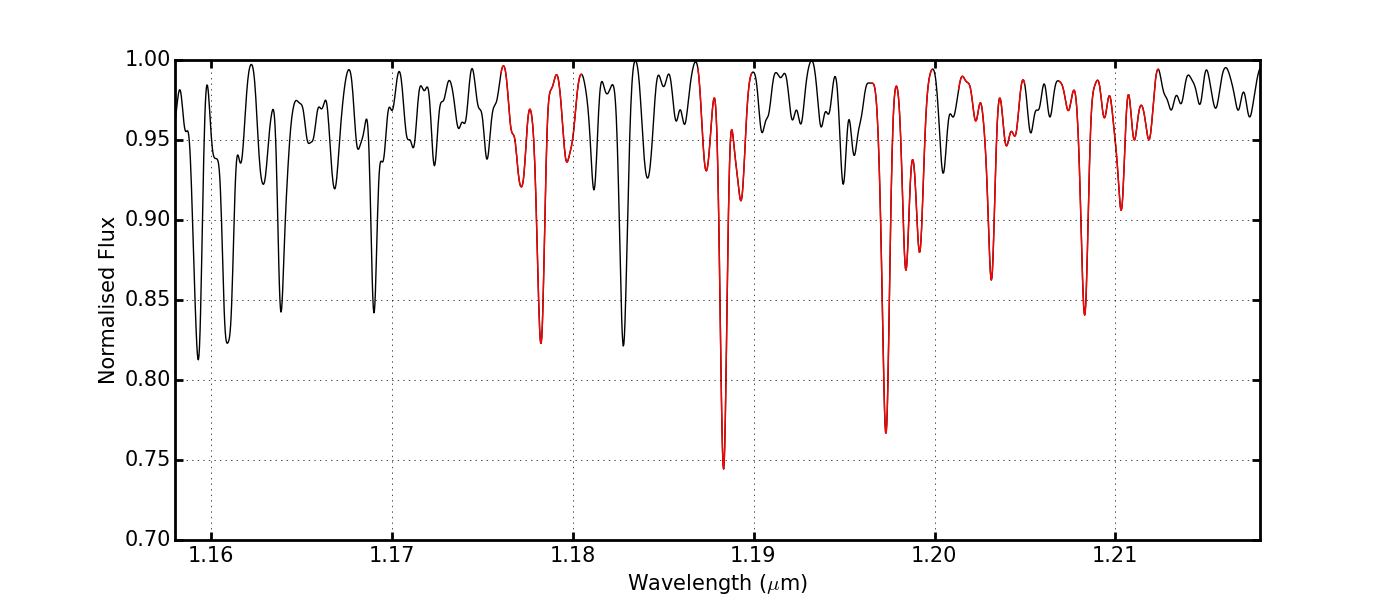
\includegraphics[width=18.0cm]{NGC2100-rv-regions}
 \caption{Sythetic RSG spectrum used calcualte the radial velocities for programme stars.
 Red regions illustrate regions where a cross-correlation is performed between the observed spectra and this synthetic spectrum.
 These regions provide consistent results with an average dispersion between the five regions of of 2.3\,\kms.
\label{fig:rv-regions}
          }
\end{figure*}


\begin{figure}
 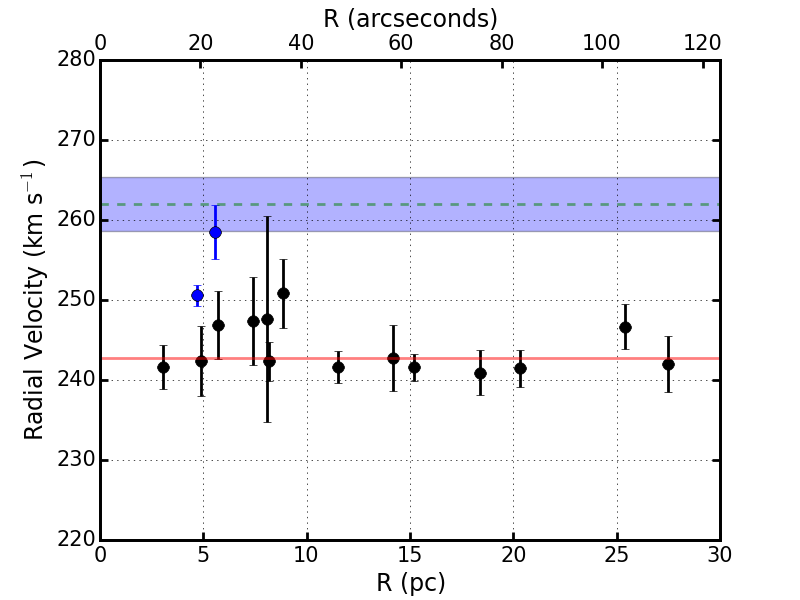
\includegraphics[width=9.0cm]{NGC2100-rv-v6}
 \caption{Radial velocities of KMOS targets shown as a function of distance from the cluster centre.
 Green dashed line shows the LMC systemtic veloctiy with the error highlighed by the blue shaded region~\citep[$262.2\pm3.4$\,\kms;][]{2012AJ....144....4M}
 and the solid red line shows the mean of the sample ($242.7\pm2.4\,$\kms).
\label{fig:rvs}
          }
\end{figure}

\begin{table*}
\caption{
        Previous radial velocity measurements in NGC\,2100.\label{tb:rvs}
        }
\scriptsize
\begin{center}
\begin{tabular}{lclll}
 \hline
 \hline
ID & ID in current study & RV (\kms) & Reference & Notes \\
 \hline
407 & ---         & $258.5\pm3.4$           & \cite{2015arXiv150803490E} &  O9.5\,II  \\
408 & ---         & $250.6\pm1.3$           & \cite{2015arXiv150803490E} &  B3\,Ia    \\
B17 & 207-0135059 & $255\pm8$/$245.0\pm2.9$ & {\cite{1994A&A...282..717J}} \\
C2  & 207-0134811 & $270\pm8$/$239.8\pm1.3$ & {\cite{1994A&A...282..717J}} & \\
C32 & 207-0135162 & $260\pm8$/$240.2\pm1.4$ & {\cite{1994A&A...282..717J}} & \\
C34 & ---         & $265\pm8$               & {\cite{1994A&A...282..717J}} & \\
NGC\,2100 & ---   & $280\pm10(16)$          & {\cite{1972MNRAS.159..445A}} & Whole cluster\\
NGC\,2100 & --- & $282.2\pm2.5$             & {\cite{1971ApJ...169..271S}} & Gas\\
NGC\,2100 & --- & $253\pm17$                & {\cite{1970PhD...........F}} & \\

\hline
\end{tabular}
\end{center}
{Value in braces is the error defined from~\cite{1983ApJ...272..488F}.}
\end{table*}

\subsection{Velocity Dispersion} % (fold)
\label{sub:velocity_dispersion}

An upper limit to the line-of-sight velocity dispersion is calculated using the equations,
\begin{equation}
  \mu = \frac{1}{\sum_{i} 1/\sigma_{i}^{2}} \sum_{i} \frac{RV_{i}}{\sigma_{i}},
\end{equation}

\begin{equation}
Var = \frac{1}{\sum_{i}1/\sigma_{i}^{2}} \sum_{i}\frac{(RV_{i} - \mu)^{2}}{\sigma_{i}^{2}},
\end{equation}

\begin{equation}
  \sigma_{1D} = \sqrt{Var \frac{N}{N - 1}},
\end{equation}

\noindent where $\sigma_{i}$ is the uncertainty on the radial velocity measurement $RV_{i}$, $\mu$ is the weighted mean and $N$ is the number of stars in the sample.
Figure~\ref{fig:sig1d} shows the line-of-sight velocity dispersion profile for RSGs in NGC\,2100.
We see that the dispersion is consistent with a flat profile with a value of $\sim$2.5\,\kms.
The apparent outlier at $\sim$5\,pc is owing to the low number statistics within this radius.
Thus, we adopt $\sigma_{1D}~=~2.4\pm0.4\,$\kms, where the error is the average error $\sigma_{1D}$ measurements of the sample, as an upper limit on the line-of-sight velocity dispersion profile of NGC\,2100.
A discussion on how binarity affects this distribution is given in Section~\ref{sub:velocity_dispersion_Mdyn}.
% As RSGs are observationally intrinsically single objects, we do not expect this dispersion to be affected significantly by binary motions, which are known to increase the dispersion profile of young massive clusters~\citep{2010MNRAS.402.1750G,2012A&A...546A..73H}.
% % \textbf{Note Gieles et al. 2010 acutally use RSGs whos binary fraction they estimate at 25\%}

% Using these equations for all stars within the sample, $\sigma_{1D}~=~3.10\pm0.11\,$\kms where the error is the average error of the radial velocities of the sample.


\begin{figure}
 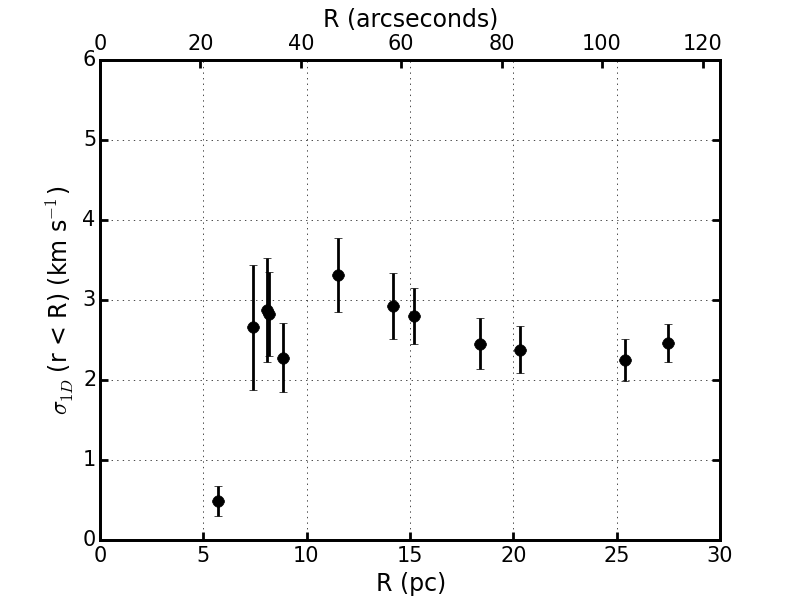
\includegraphics[width=9.0cm]{NGC2100-sig1d-v6}
 \caption{Observed line-of-sight velocity dispersion as a function of the distance from the centre of NGC\,2100.
\label{fig:sig1d}
          }
\end{figure}


% subsection velocity_dispersion (end)

\subsection{Dynamical Mass} % (fold)
\label{sub:dynamical_mass}


Using $\sigma_{1D}$ as an upper limit on the velocity distribution, one can calculate the dynamical mass of the cluster using the virial equation,

\begin{equation}
  M_{dyn} = \frac{\eta\sigma_{1D}^{2}r_{eff}}{G},
  \label{eq:vir}
\end{equation}

\noindent where $M_{dyn}$ is the virial mass, $\eta~=~6r_{vir}/r_{eff}~=~9.75$ providing the density profile of the cluster is sufficiently steep~\citep{2010ARA&A..48..431P}.
However, NGC\,2100 has a relatively shallow density profile ($\gamma~=~2.3$) which means $\eta>9.75$ therefore the estimate of $M_{dyn}$ is knowingly an overestimate.
Using $\sigma_{1D}~=~2.4\pm0.4$\,\kms and equation~\ref{eq:vir}, the dynamical mass of NGC\,2100 is $M_{dyn}~=~(5.8\pm2.0)\times 10^{4}M_{\odot}$.
Comparing this to the photometric mass $M_{phot}~=~(2.3\pm1.0)\times 10^{4}M_{\odot}$~\citep{2005ApJS..161..304M} we see that the dynamical mass appears to be a barely significant overestimate.
\citet{2010MNRAS.402.1750G} explain this discrepancy by demonstrating that binary motions can increase the measured velocity dispersion profile.
\citet{2012A&A...546A..73H} note that had binarity been neglected they would have measured a $\sigma_{1D}$ a factor of five higher for R136.
% is larger, which is expected owing to binary motions within the cluster~\citep{2010MNRAS.402.1750G}.
However, the mean lifetime for RSGs within binary systems is significantly decreased~\citep{2008MNRAS.384.1109E}.
These authors also note that where mass transfer occurs, the number of RSGs drastically decreases.
We can therefore expect that the numbers of RSGs in a close binary system are very small~\cite{2009ApJ...696.2014D}.

Therefore, the velocity dispersion profile derived using an effectively single sample of RSGs should not be affected by binary motions.
This leads to the conclusion that the only factor affecting the estimation of $M_{dyn}$ is the $\eta$ parameter.
Using a lower limit of $\eta~=~7.0$~\citep[estimated from Fig. 4a from ][]{2010ARA&A..48..431P}, $M_{dyn}~=~(4.2\pm1.4)\times 10^{4}M_{\odot}$ which still lies above the photometric mass however with a low significance.
Why this is the case is addressed in section~\ref{sec:discussion}.


% subsection dynamical_mass (end)


% section radial_velocities (end)

\subsection{Stellar Parameters} % (fold)
\label{sub:stellar_parameters}

Stellar parameters are estimated using the J-band analysis technique described initially in~\cite{2010MNRAS.407.1203D}
and tested rigorously in~\cite{2014ApJ...788...58G} and~\cite{2015ApJ...806...21D}.
These studies show that using a narrow spectral window within the $J$-band one can accurately derive global metallicity ([Z]) to within
$\pm0.2\,dex$ at the resolution of KMOS observations with S/N~$\ge~100$.
\cite{2015ApJ...803...14P} builds on this by demonstrating the feasibility of this technique using KMOS spectra.

This analysis uses synthetic RSG spectra, extracted from {\sc marcs} model atmospheres~\citep{2008A&A...486..951G}, computed with non-local thermodynamic equilibrium corrections for stellar lines for titanium, iron, silicon and magnesium~\citep{2012ApJ...751..156B,2013ApJ...764..115B,2015ApJ...804..113B}.
The parameter ranges for the grid of synthetic RSG spectra are listed in Table~\ref{tb:mod_range}.
The synthetic spectra are compared with observations using a $\chi$-squared minimisation approach where the synthetic spectra are degraded to the resolution and sampling of the observations.

Estimated stellar parameters are listed in Table~\ref{tb:stellar-params}.
Reliable parameters could not be estimated for two stars (0207-0135059 and 0207-0135206).
Figure~\ref{fig:model_fits} shows the observed KMOS spectra (black) along with each best-fitting model spectrum (red).
The average metallicity for the 11 stars within NGC\,2100 is $-0.30\pm0.11\,dex$ and the distribution of metals with respect to distance from the cluster centre is shown in Figure~\ref{fig:ZvsR}.
This figure shown no evidence for a spatial distribution of metallicity across the extent of the cluster.


The average metallicity in NGC\,2100 compares well to estimates of the cluster metallicity using isochrone fitting to the optical colour-magnitude diagram~\citep[$-0.34\,dex$;][]{2015A&A...575A..62N}.
The only other estimate of stellar metallicity within this cluster comes from~\cite{1994A&A...282..717J}
who estimate metallicities using optical spectroscopy of four RSGs.
This study finds an average metallicity for NGC\,2100 $-0.32\pm0.03\,dex$ which our estimate agrees well with.

Using the same analysis technique as used in this study,~\cite{2015ApJ...806...21D} estimate metallicities for nine RSGs within the LMC, finding an average value of $-0.37\pm0.14\,dex$ which again,
our estimate agrees well with.


\begin{figure*}
 %\vspace{302pt}
 \begin{center}
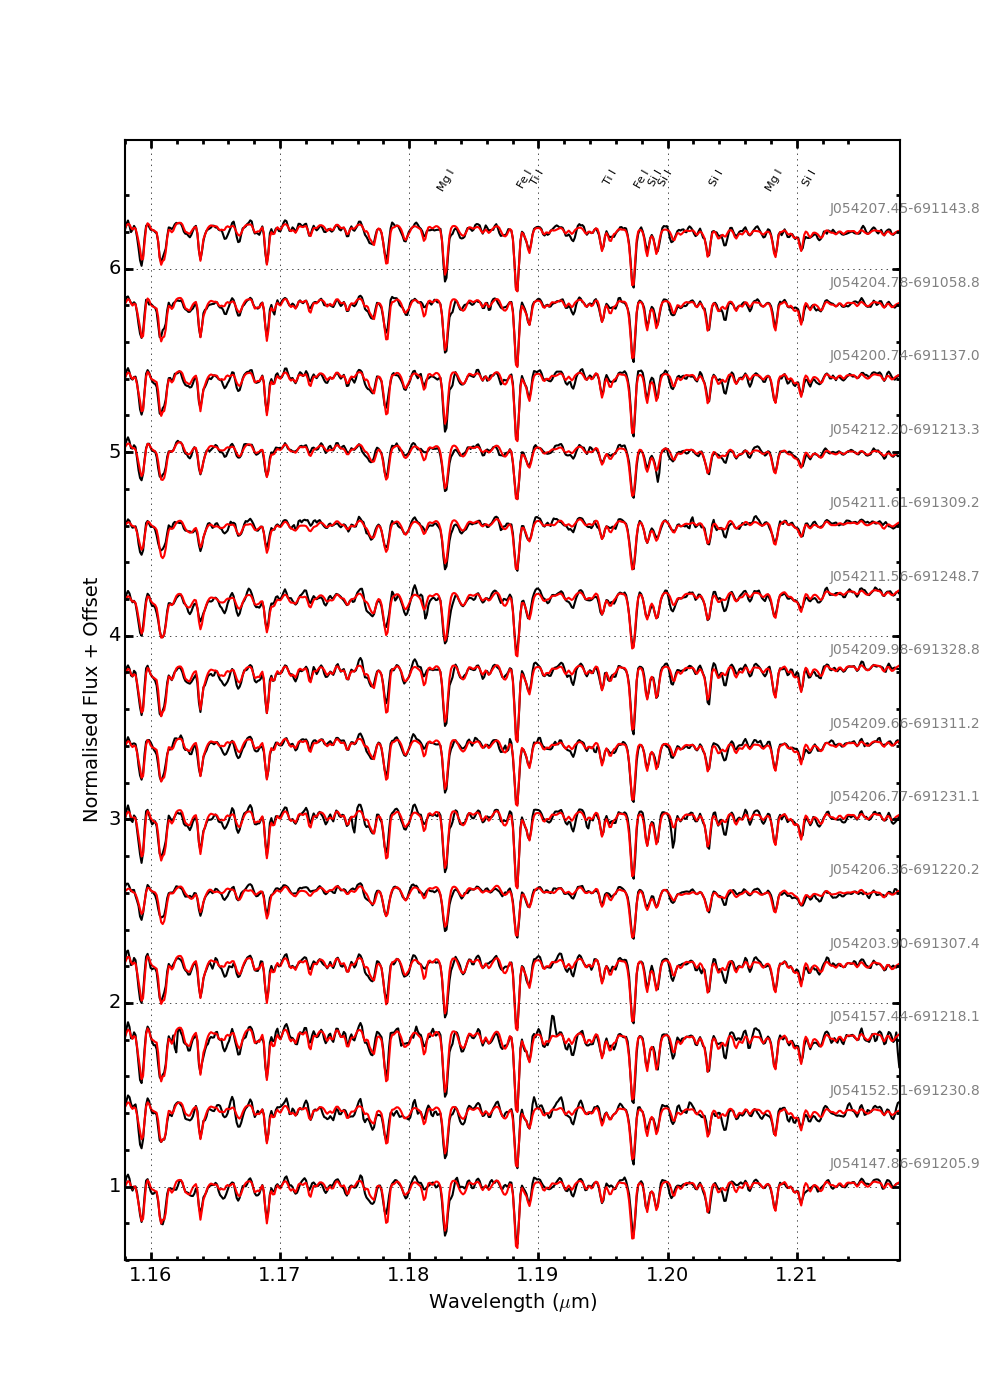
\includegraphics[width=16cm]{NGC2100-model-fits}
\caption{KMOS spectra of the NGC\,2100 RSGs and their associated best-fit model spectra
(black and red lines, respectively).
The lines used for the analysis from left-to-right by species are:
Fe\,I$\lambda\lambda$1.188285,
1.197305,
Si\,I$\lambda\lambda$1.198419,
1.199157,
1.203151,
1.210353,
Ti\,I$\lambda\lambda$1.189289,
1.194954.
         }
\label{fig:model_fits}
\end{center}
\end{figure*}




\begin{figure}
 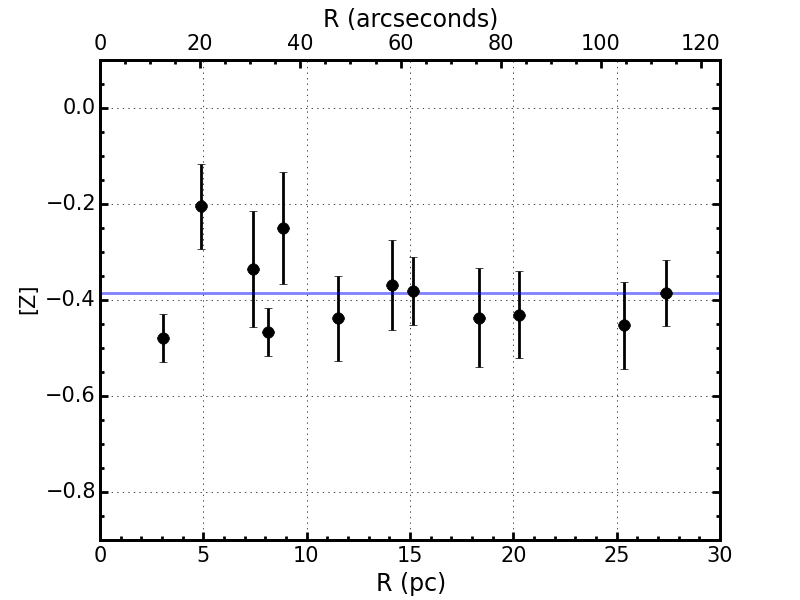
\includegraphics[width=9.0cm]{NGC2100-ZvsR}
 \caption{Estimated metallicities shown against distance from the centre of the cluster where the solid blue line denotes the mean of the sample $-0.3\pm0.11\,dex$.
\label{fig:ZvsR}
          }
\end{figure}

\begin{table}
\caption{
Model grid used for analysis.\label{tb:mod_range}
         }
\scriptsize
\begin{center}
\begin{tabular}{lccc}
 \hline
 \hline
  Model Parameter & Min. & Max. & Step size \\
 \hline
T$_{eff}$ (K)        & 3400 & 4400 & 100 \\
$[$Z$]$ (dex)   & $-$1.0\o & 1.0\o  & 0.1\o\\
log\,$g$ (cgs)  & $-$1.00 & 1.00 & 0.25\\
 $\xi$ (\kms)  & \pp1.0\o & 5.0\o & 0.2\o\\
 \hline
\end{tabular}
\end{center}
\end{table}

\begin{table*}
\begin{center}
\caption{
Fit parameters for NGC\,2100 KMOS targets
\label{tb:stellar-params}
         }
\scriptsize
\begin{tabular}{lc ccccc}
 \hline
 \hline
  Target  & IFU & $\xi$ (\kms) & [Z] & log\,$g$ & T$_{eff}$ (K) & Notes\\
  \hline
0207-0134568 & 7  & 3.8 $\pm$ 0.3 &  -0.36 $\pm$ 0.10 & 0.50 $\pm$ 0.09 & 4017 $\pm$ 55  & \\
0207-0134683 & 9  & 3.6 $\pm$ 0.3 &  -0.33 $\pm$ 0.15 & 0.96 $\pm$ 0.38 & 4100 $\pm$ 71  & \\
0207-0134811 & 6  & 5.0 $\pm$ 0.1 &  -0.21 $\pm$ 0.09 & 0.67 $\pm$ 0.17 & 4084 $\pm$ 47  & C2\\
0207-0134979 & 12 & 4.4 $\pm$ 0.3 &  -0.25 $\pm$ 0.10 & 0.74 $\pm$ 0.12 & 4000 $\pm$ 31  & \\
0207-0135059 & 24 & 2.2 $\pm$ 0.8 &   0.32 $\pm$ 0.42 & 0.85 $\pm$ 0.11 & 3715 $\pm$ 181 & B17\\
0207-0135069 & 10 & 4.9 $\pm$ 0.1 &  -0.30 $\pm$ 0.08 & 0.70 $\pm$ 0.12 & 4013 $\pm$ 37  & \\
0207-0135150 & 14 & 4.1 $\pm$ 0.3 &  -0.37 $\pm$ 0.13 & 0.73 $\pm$ 0.14 & 3900 $\pm$ 57  & \\
0207-0135162 & 11 & 5.0 $\pm$ 0.1 &  -0.28 $\pm$ 0.08 & 0.70 $\pm$ 0.19 & 4024 $\pm$ 43  & C32\\
0207-0135205 & 20 & 4.2 $\pm$ 0.3 &  -0.24 $\pm$ 0.12 & 0.50 $\pm$ 0.09 & 3896 $\pm$ 61  & \\
0207-0135206 & 18 & 2.0 $\pm$ 0.4 &   0.56 $\pm$ 0.23 & 1.00 $\pm$ 0.00 & 3671 $\pm$ 104 & \\
0207-0135220 & 22 & 3.6 $\pm$ 0.4 &  -0.24 $\pm$ 0.17 & 1.00 $\pm$ 0.12 & 4034 $\pm$ 50  & \\
0208-0135292 & 4  & 4.3 $\pm$ 0.3 &  -0.34 $\pm$ 0.10 & 0.75 $\pm$ 0.10 & 3947 $\pm$ 50  & \\
0208-0135383 & 3  & 4.2 $\pm$ 0.3 &  -0.35 $\pm$ 0.11 & 0.91 $\pm$ 0.16 & 3965 $\pm$ 50  & \\
0208-0135446 & 2  & 4.1 $\pm$ 0.3 &  -0.33 $\pm$ 0.15 & 0.97 $\pm$ 0.11 & 3911 $\pm$ 67  & \\

  \hline
  \end{tabular}
  \end{center}
\end{table*}

% section stellar_parameters (end)

\section{Discussion} % (fold)
\label{sec:discussion}
% \begin{itemize}
%   \item Do these Teff's fit into the picture?
%   \item Can we believe the Z's?
%   \item Can we say anything about an age spread? (Niederhofer et al. 2015)
%   \item e.g. is the distribution of masses what we would expect from a cluster with a single stellar population?
%   \item Given the small range in luminosities, probably!
%   \item Compare to PerOB1
% \end{itemize}


\subsection{Stellar Parameters} % (fold)
\label{sub:stellar_parameters_disc}
As mentioned previously, JT94 measure stellar parameters for four RSGs using optical spectroscopy.
These authors measure effective temperature, $log\,g$, microturblence and metallicities for each star by comparing their spectra to a set of synthetic spectra.
A method not dissimilar to out own.
We find that there are three targets in common with our study: B17, C2, C32.
Comparing results we find \textbf{that unbelievably, all of the targets in common have problems with their fits! (5 stars have issues with their fits, in total, and three of them are in this sample! To say more on this I need to identify why exactly these fits are perturbed.)}

When we compare the average values taken from JT94 where we find excellent agreement for all parameters apart from surface gravity where our estimates are within 2$\sigma$ of the previous estimates, however, as this is not a significant outlier no further discussion will be made of this and it will suffice to say that, to within the uncertainties on average our results compare well to previous estimates.

% For reference:\\
% JT94 Teff: $4081\pm75$, $log\,g$: $0.4\pm0.2$, $\xi$: 4.5~\cite[no error quoted in][]{1994A&A...282..717J}.\\
% Our values: Teff: $3991\pm15$, $log\,g$: $0.76\pm0.05$, $\xi$: $4.26\pm0.08$

Luminosities have been estimated using the bolometric correction in~\cite{2013ApJ...767....3D} and a H-R diagram for the clusters is presented in Figure~\ref{fig:HRD}.
Overlaid on this H-R diagram are {\sc syclist} stellar isochrones for both SMC-like~\citep[solid lines][]{2013A&A...558A.103G} and solar-like~\citep[dashed lines][]{} at various ages where stellar rotation is 40\% of the critical velocity.


% The narrow range in masses implied by the luminosities of the stars (regardless of which evolutionary models is used) adds strength to the argument that these stars were all formed in a single burst of star formation.

\begin{figure}
 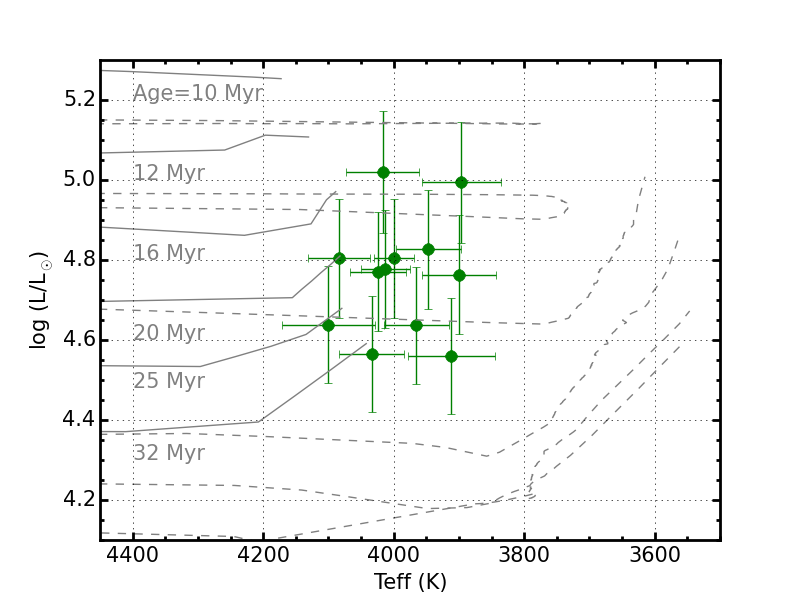
\includegraphics[width=9.0cm]{NGC2100-HRD-iso}
 \caption{H-R diagram for 12 RSGs in NGC2100.
  Bolometric corrections computed using~\citet{2013ApJ...767....3D}.
  Cluster isochrones from~\citet{2013A&A...558A.103G} are overlaid in grey at a metallicity of $Z~=~-0.85\,dex$ without stellar rotation at ages of 10...30\,Myrs.
\label{fig:HRD}
          }
\end{figure}

In Figure~\ref{fig:TeffvsZ} we compare the estimated effective temperatures and metallicities with those derived for RSGs within the LMC~\citep{2015ApJ...806...21D}.
This figure shows that the range in metallicities and temperatures estimated in this study compares well with those derived in~\cite{2015ApJ...806...21D}.

\begin{figure}
 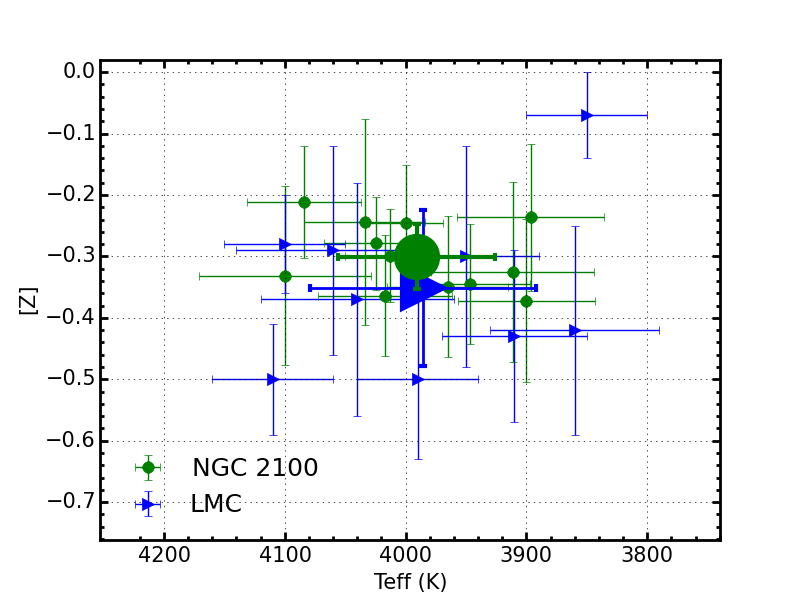
\includegraphics[width=9.0cm]{NGC2100-TeffvsZ-2100-LMC}
 \caption{Estimated metallicities shown against estimated effective temperature.
\label{fig:TeffvsZ}
          }
\end{figure}
% subsection stellar_parameters (end)
\subsection{Velocity Dispersion and Dynamical Mass} % (fold)
\label{sub:velocity_dispersion_Mdyn}
% The argument for binary motions pumping up sig1D follows like this:
% \begin{itemize}
%   \item Undetected binaries within the sample act to increase the sig1D of the cluster
%   \item This then drives up the mass derived using equation~\ref{eq:vir}
%   \item Could we estimate the binary fraction among RSGs in this cluster?
%   \item I have always been told/assumed that binary fraction among RSGs is low.
%   \item If the binary fraction is low/0. Could binaires really be the reason we see a larger sig1d? Super virial?
% \end{itemize}


This study represents the first estimate of the line-of-sight velocity dispersion profile for NGC\,2100.
Comparing the estimated velocity dispersion of NGC\,2100 with that of other young massive clusters in the Local Universe is useful to ascertain whether this cluster shares similar properties to other more well studied young massive clusters.
We find the dynamical properties NGC\,2100 is well matched by other clusters with similar masses and ages, particularly so with RSGC02, a Galactic young massive cluster.
Below we compare the dynamical results for NGC\,2100 to that of several young massive clusters first within the LMC and then within the Galaxy.

\subsubsection{Comparison with LMC clusters} % (fold)
\label{sub:comparison_with_lmc_clusters}


The line-of-sight velocity dispersion profile of the young massive cluster R136 has been estimated at 6\,\kms~\citep{2012A&A...546A..73H} using multi-epoch spectroscopy from the VLT-Flames Tarantula Survey~\citep{2011A&A...530A.108E}.
NGC\,2100 and R136 are both located within the 30 Doradus region and within the LMC\,2 supershell.
R136 is around twice as massive as NGC\,2100 with the photometric mass of R136 being estimated at $\sim10^{5}M_{\odot}$ with an age less than 2\,Myr~\citep{1998ApJ...509..879D,1998ApJ...493..180M,2010MNRAS.408..731C}.
This makes R136 significantly younger than NGC\,2100 ($\sim20$\,Myr) and it is therefore unsurprising that the velocity dispersion profile is larger for R136 as one would expect a massive cluster to relax over time.

NGC\,1850 is a young LMC massive cluster with a photometric mass of $1.4\times10^{5}$ and a recently revised age of $93\,Myr$~\citep{2015A&A...575A..62N}.
\citet{2005ApJS..161..304M} report a line-of-sight velocity dispersion for this cluster as $3.0\pm0.7\,$\kms which compares well to the dispersion in NGC\,2100 even though this cluster is significantly older are more massive.

NGC\,2004 is a young massive cluster in the LMC with a mass and age similar to that of NGC\,2100~\citep[20\,Myr; $2\times10^{4}M_{\odot}$][and references therein]{2015A&A...575A..62N}.
\citet{2006A&A...456..623E} obtained multi-epoch spectra for massive stars within this cluster and derive radial velocities without however dynamical analysis of the cluster.
This cluster has remarkably similar properties to NGC\,2100 and therefore a comparison between their dynamical properties is useful to the intrinsic distribution of dynamical properties within young massive clusters.

% subsubsection comparison_with_lmc_clusters (end)

\subsubsection{Comparison with Galactic Clusters} % (fold)
\label{sub:galactic_clusters}

RSGC01 is a cluster with a large population of RSGs within the Galaxy~\citep{2007ApJ...671..781D}.
This cluster is shown to have a mass $\sim3\times10^{4}M_{\odot}$ with an age 17\,Myr and a velocity dispersion of 2.8\,\kms.
Therefore this cluster compares remarkably well with NGC\,2100.

Westerlund\,1 is a massive young star cluster in the Galaxy with a large population of massive stars~\citep{2005A&A...434..949C}.
This cluster is young compared to NGC\,2100 with an age of 3.5\,Myr therefore many of the stars which will become RSGs in the future are currently fusing hydrogen on the main sequence.
The photometric mass of Westerlund\,1 is $\sim3\times10^{4}M_{\odot}$ with a measured velocity dispersion of 5.8\,\kms.
Like R136 in the LMC, Westerlund1\,1 has a higher velocity dispersion and a young age.

% subsubsection galactic_clusters (end)

% subsection velocity_dispersion (end)

% \subsection{Distribution of RSGs} % (fold)
% \label{sub:distribution_of_rsgs}
% \begin{itemize}
%   \item Why are many of the RSGs so far away from the cluster centre?
%   \item Core radius is 3.0pc which means these RSGs are out to 10x the core radius. Is that unusual?
% \end{itemize}
% subsection distribution_of_rsgs (end)

% section discussion (end)

\section{Conclusions} % (fold)
\label{sec:conclusions}

Using KMOS spectra of 14 RSGs in NGC\,2100 we have for the fist time estimated the dynamical properties of this young massive cluster.
Radial velocities have been estimated using KMOS to a precision of $\sim1$\,\kms, demonstrating that this instrument can be used to study the dynamical properties of stars in external galaxies.

The line-of-sight velocity dispersion profile has been estimated in Figure~\ref{fig:sig1d} and has been shown to be flat outside 10\,pc from the cluster centre.
A low velocity dispersion of $\sigma_{1D}~=~3.01\pm0.11\,$\kms has been adopted and NGC\,2100 has therefore been shown to be in virial equilibrium.
This adds evidence to the theory that young star clusters appear to remain in virial equilibrium from an early age and hence expand owing to stellar evolution of a relatively slow timescales (10Myr; SPZ10).
We compare the velocity dispersion profiles of other young massive clusters in the LMC and the Galaxy and find that the distribution of velocity dispersions is consistent with this evolution.
\textbf{Need to illustrate this with a Mass/Age vs sig figure.}

Characterisation of the velocity dispersion profile for the cluster allows for the first time the dynamical mass to be estimated (assuming virial equilibrium) as $log(M_{dyn}/M_{\odot})~>~4.8$.
A discussion of the appropriate value of $\eta$ for this cluster is detailed in Section~\ref{sub:dynamical_mass}.

We also derive stellar parameters using the $J$-band analysis technique~\citep{2010MNRAS.407.1203D} for all targets within the sample and show that the estimated parameters agree well with previous studies within the LMC~\citep{2015ApJ...806...21D}.
Using temperatures from the analysis technique we construct a H-R diagram of RSGs within NGC\,2100 and estimate the age of the cluster using isochrones fitting~\citep{2013A&A...558A.103G} (Ekstrom12) to be $20\pm5\,$Myr, in good agreement with previous estimate of this cluster~\citep{2015A&A...575A..62N}.



% section conclusions (end)
\section*{Acknowledgements}

...
% \bibliographystyle{mn2e}                      % The reference style
\bibliography{journals}
% \bibliography{journals}

\begin{thebibliography}{99}

\bibitem[Andrews
\& Lloyd Evans(1972)]{1972MNRAS.159..445A} Andrews, P.~J., \& Lloyd Evans, T.\ 1972, \mnras, 159, 445

\bibitem[Bergemann et al.(2012)]{2012ApJ...751..156B} Bergemann, M.,
Kudritzki, R.-P., Plez, B., et al.\ 2012, \apj, 751, 156

\bibitem[Bergemann et al.(2013)]{2013ApJ...764..115B} Bergemann, M.,
Kudritzki, R.-P., W{\"u}rl, M., et al.\ 2013, \apj, 764, 115

\bibitem[Bergemann et al.(2015)]{2015ApJ...804..113B} Bergemann, M.,
Kudritzki, R.-P., Gazak, Z., Davies, B., \& Plez, B.\ 2015, \apj, 804, 113

\bibitem[Clark et
al.(2005)]{2005A&A...434..949C} Clark, J.~S., Negueruela, I., Crowther, P.~A., \& Goodwin, S.~P.\ 2005, \aap, 434, 949

\bibitem[Crowther et al.(2010)]{2010MNRAS.408..731C} Crowther, P.~A.,
Schnurr, O., Hirschi, R., et al.\ 2010, \mnras, 408, 731

\bibitem[Davies et al.(2007)]{2007ApJ...671..781D} Davies, B., Figer,
D.~F., Kudritzki, R.-P., et al.\ 2007, \apj, 671, 781

\bibitem[Davies et al.(2009)]{2009ApJ...696.2014D} Davies, B., Origlia, L.,
Kudritzki, R.-P., et al.\ 2009, \apj, 696, 2014

\bibitem[Davies et al.(2010)]{2010MNRAS.407.1203D} Davies, B., Kudritzki,
R.-P., \& Figer, D.~F.\ 2010, \mnras, 407, 1203

\bibitem[Davies et al.(2013)]{2013ApJ...767....3D} Davies, B., Kudritzki,
R.-P., Plez, B., et al.\ 2013, \apj, 767, 3

\bibitem[Davies et al.(2015)]{2015ApJ...806...21D} Davies, B., Kudritzki,
R.-P., Gazak, Z., et al.\ 2015, \apj, 806, 21

\bibitem[Davies et
al.(2013)]{2013A&A...558A..56D} Davies, R.~I., Agudo Berbel, A., Wiezorrek, E., et al.\ 2013, \aap, 558, A56

\bibitem[de Koter et al.(1998)]{1998ApJ...509..879D} de Koter, A., Heap,
S.~R., \& Hubeny, I.\ 1998, \apj, 509, 879

\bibitem[Eldridge et al.(2008)]{2008MNRAS.384.1109E} Eldridge, J.~J.,
Izzard, R.~G., \& Tout, C.~A.\ 2008, \mnras, 384, 1109

\bibitem[Elson(1991)]{1991ApJS...76..185E} Elson, R.~A.~W.\ 1991, \apjs,
76, 185

\bibitem[Evans et
al.(2006)]{2006A&A...456..623E} Evans, C.~J., Lennon, D.~J., Smartt, S.~J., \& Trundle, C.\ 2006, \aap, 456, 623

\bibitem[Evans et
al.(2011)]{2011A&A...530A.108E} Evans, C.~J., Taylor, W.~D., H{\'e}nault-Brunet, V., et al.\ 2011, \aap, 530, A108

\bibitem[Evans et al.(2015)]{2015arXiv150803490E} Evans, C.~J., van Loon,
J.~T., Hainich, R., \& Bailey, M.\ 2015, arXiv:1508.03490

\bibitem [Ford(1970)]{1970PhD...........F} Ford, H., 1970, PhD. Thesis, University of Wisconsin.

\bibitem[Freeman et al.(1983)]{1983ApJ...272..488F} Freeman, K.~C.,
Illingworth, G., \& Oemler, A., Jr.\ 1983, \apj, 272, 488

\bibitem[Gazak et al.(2013)]{2013MNRAS.430L..35G} Gazak, J.~Z., Bastian,
N., Kudritzki, R.-P., et al.\ 2013, \mnras, 430, L35

\bibitem[Gazak et al.(2014)]{2014ApJ...788...58G} Gazak, J.~Z., Davies, B.,
Kudritzki, R., Bergemann, M., \& Plez, B.\ 2014, \apj, 788, 58

\bibitem[Gazak et al.(2014)]{2014ApJ...787..142G} Gazak, J.~Z., Davies, B.,
Bastian, N., et al.\ 2014, \apj, 787, 142

\bibitem[Gazak et al.(2015)]{2015ApJ...805..182G} Gazak, J.~Z., Kudritzki,
R., Evans, C., et al.\ 2015, \apj, 805, 182

\bibitem[Georgy et
al.(2013)]{2013A&A...558A.103G} Georgy, C., Ekstr{\"o}m, S., Eggenberger, P., et al.\ 2013, \aap, 558, A103

\bibitem[Gieles et al.(2010)]{2010MNRAS.402.1750G} Gieles, M., Sana, H.,
\& Portegies Zwart, S.~F.\ 2010, \mnras, 402, 1750

% \bibitem[Glatt et
% al.(2010)]{2010A&A...517A..50G} Glatt, K., Grebel, E.~K., \& Koch, A.\ 2010, \aap, 517, A50

\bibitem[Gratton et
al.(2012)]{2012A&A...539A..19G} Gratton, R.~G., Lucatello, S., Carretta, E., et al.\ 2012, \aap, 539, A19

\bibitem[Gustafsson et
al.(2008)]{2008A&A...486..951G} Gustafsson, B., Edvardsson, B., Eriksson, K., et al.\ 2008, \aap, 486, 951

\bibitem[H{\'e}nault-Brunet et
al.(2012)]{2012A&A...546A..73H} H{\'e}nault-Brunet, V., Evans, C.~J., Sana, H., et al.\ 2012, \aap, 546, A73

\bibitem[Jasniewicz
\& Thevenin(1994)]{1994A&A...282..717J} Jasniewicz, G., \& Thevenin, F.\ 1994, \aap, 282, 717

\bibitem[King(1966)]{1966AJ.....71...64K} King, I.~R.\ 1966, \aj, 71, 64

\bibitem[Lada
\& Lada(2003)]{2003ARA&A..41...57L} Lada, C.~J., \& Lada, E.~A.\ 2003, \araa, 41, 57

\bibitem[Lapenna et al.(2015)]{2015ApJ...798...23L} Lapenna, E., Origlia,
L., Mucciarelli, A., et al.\ 2015, \apj, 798, 23

\bibitem[Longmore et al.(2014)]{2014prpl.conf..291L} Longmore, S.~N.,
Kruijssen, J.~M.~D., Bastian, N., et al.\ 2014, Protostars and Planets VI,
291

\bibitem[Massey
\& Hunter(1998)]{1998ApJ...493..180M} Massey, P., \& Hunter, D.~A.\ 1998, \apj, 493, 180

\bibitem[McConnachie(2012)]{2012AJ....144....4M} McConnachie, A.~W.\ 2012,
\aj, 144, 4

\bibitem[McLaughlin
\& van der Marel(2005)]{2005ApJS..161..304M} McLaughlin, D.~E., \& van der Marel, R.~P.\ 2005, \apjs, 161, 304

\bibitem[Miller et al.(1997)]{1997AJ....114.2381M} Miller, B.~W., Whitmore,
B.~C., Schweizer, F., \& Fall, S.~M.\ 1997, \aj, 114, 2381

\bibitem[Niederhofer et
al.(2015)]{2015A&A...575A..62N} Niederhofer, F., Hilker, M., Bastian, N., \& Silva-Villa, E.\ 2015, \aap, 575, A62

\bibitem[Patrick et al.(2015)]{2015ApJ...803...14P} Patrick, L.~R., Evans,
C.~J., Davies, B., et al.\ 2015, \apj, 803, 14

\bibitem[Points et al.(1999)]{1999ApJ...518..298P} Points, S.~D., Chu,
Y.~H., Kim, S., et al.\ 1999, \apj, 518, 298

\bibitem[Portegies Zwart et
al.(2010)]{2010ARA&A..48..431P} Portegies Zwart, S.~F., McMillan, S.~L.~W., \& Gieles, M.\ 2010, \araa, 48, 431

\bibitem[Robertson(1974)]{1974A&AS...15..261R} Robertson, J.~W.\ 1974, \aaps, 15, 261

\bibitem[Smith
\& Weedman(1971)]{1971ApJ...169..271S} Smith, M.~G., \& Weedman, D.~W.\ 1971, \apj, 169, 271

\bibitem[Whitmore
\& Schweizer(1995)]{1995AJ....109..960W} Whitmore, B.~C., \& Schweizer, F.\ 1995, \aj, 109, 960

\bibitem[Zepf et al.(1999)]{1999AJ....118..752Z} Zepf, S.~E., Ashman,
K.~M., English, J., Freeman, K.~C., \& Sharples, R.~M.\ 1999, \aj, 118, 752
\end{thebibliography}
\label{lastpage}

\end{document}
